\title{CS 613 - Machine Learning}
\author{Assignment 3 - Classification)\\ 	Alex Lapinski\\ 	Fall 2016}
\date{11/6/2016}
\documentclass[12pt]{article}
\usepackage[margin=0.7in]{geometry}
\usepackage{graphicx}
\usepackage{float}
\usepackage{comment}
\usepackage{amsmath}
\usepackage{hyperref}
\graphicspath{ {images/} }
\hypersetup{
	colorlinks=true,
	linkcolor=blue,
	filecolor=magenta,
	urlcolor=cyan
}
\urlstyle{same}
\begin{document}
\maketitle
\section{Theory}
\begin{enumerate}
\item Consider the following set of training examples for an unknown target function:  $(x_1, x_2)\rightarrow y$:
\begin{table}[h]
\begin{center}
\begin{tabular}{|l|l|l|l|}
\hline
Y & $x_1$ & $x_2$ & Count\\
\hline
+ & T & T & 3\\
+ & T & F & 4\\
+ & F & T & 4\\
+ & F & F & 1\\
- & T & T & 0\\
- & T & F & 1\\
- & F & T & 3\\
- & F & F & 5\\
\hline
\end{tabular}
\end{center}
\end{table}
\begin{enumerate}
\item What is the sample entropy, $H(Y)$ from this training data (using log base 2) (2pts)?
\hfill \linebreak
\hfill \linebreak
Number of samples with '+' class (p): 12\\
Number of samples with '-' class (n): 9\\
Total number of samples (p+n): 21\\
\hfill \linebreak
\begin{equation*}
\begin{split}
		H(\frac{p}{p+n},\frac{n}{p+n})  & = H(\frac{12}{21},\frac{9}{21}) \\
		& = (-\frac{12}{21}*log_2(\frac{12}{21}) + (-\frac{9}{21}*log_2\frac{9}{21})) \\
		& = (-0.57*log_2(0.57)) + (-0.43log_2(-0.43)) \\
	         & = (-0.57*-0.81) + (-0.43 * -1.22) \\
		& = 0.46 + 0.52 \\
		& = \textbf{0.98}
\end{split}
\end{equation*}
\newpage
\item What are the information gains for branching on variables $x_1$ and $x_2$ (4pts)?
\hfill\linebreak
\hfill\linebreak
We'll first compute the information gain on $x_1$ and then on $x_2$.\\
The count for each class when split on $x_1$:
\begin{align*}
	p_{T} &= 3 + 4 = 7 & n_{T} &= 0 + 1 = 1 & p_{T} + n_{T} & = 8\\
	p_{F} &= 4 + 1 = 5 & n_{F} &= 3 + 5 = 8 & p_{F} + n_{F} & = 13 \\
	p+n &= 21 & &\\
\end{align*}
\begin{equation*}
\begin{split}
remainder(x_1) & = \frac{p_T + n_T}{p + n} * H(\frac{p_T}{p_T+n_T},\frac{n_T}{p_T+n_T}) + 
			     \frac{p_F+n_F}{p+n}*H(\frac{p_F}{p_F+n_F},\frac{n_F}{p_F+n_F})\\
	& = \frac{8}{21}*H(\frac{7}{8},\frac{1}{8}) + \frac{13}{21}*H(\frac{5}{13},\frac{8}{13})\\
	& = \frac{8}{21}*(-\frac{7}{8}*log_{2}(\frac{7}{8})-\frac{1}{8} * log_{2}(\frac{1}{8})) + 
	       \frac{13}{21}*(-\frac{5}{13}*log_{2}(\frac{5}{13})-\frac{8}{13}*log_{2}(\frac{8}{13}))\\
	& = \frac{8}{21}*(0.17+0.38) + \frac{13}{21}*(0.52+0.43)\\
	& = 0.21 + 0.59 = \textbf{0.8}\\
	\end{split}
\end{equation*}
\begin{equation*}
	IG(x_{1}) = 0.98 - 0.8 = \textbf{0.18}
\end{equation*}
\hfill\linebreak
The count for each class when split on $x_2$:
\begin{align*}
		p_{T} &= 3 + 4 = 7 & n_{T} &= 0 + 3 = 3 & p_{T} + n_{T} & = 10\\
		p_{F} &= 4 + 1 = 5 & n_{F} &= 1 + 5 = 6 & p_{F} + n_{F} & = 11\\
		p+n &= 21 & &\\
\end{align*}
\begin{equation*}
\begin{split}
	remainder(x_2) & = \frac{p_T + n_T}{p + n} * H(\frac{p_T}{p_T+n_T},\frac{n_T}{p_T+n_T}) + 
				      \frac{p_F+n_F}{p+n}*H(\frac{p_F}{p_F+n_F},\frac{n_F}{p_F+n_F})\\
	& = \frac{10}{21}*H(\frac{7}{10},\frac{3}{10}) + \frac{11}{21}*H(\frac{5}{11},\frac{6}{11})\\
	& = \frac{10}{21}*(-\frac{7}{10}*log_{2}(\frac{7}{10})-\frac{3}{10} * log_{2}(\frac{3}{10})) + 
	       \frac{11}{21}*(-\frac{5}{11}*log_{2}(\frac{5}{11})-\frac{6}{11}*log_{2}(\frac{6}{11}))\\
	& = \frac{10}{21}*(0.36+0.54) + \frac{11}{21}*(0.51+0.48)\\
	& = 0.43 + 0.52 = \textbf{0.85}\\
\end{split}
\end{equation*}
\begin{equation*}
	IG(x_{2}) = 0.98 - 0.85 = \textbf{0.13}
\end{equation*}
\hfill\newline
\newpage
\item Draw the decision tree that would be learned by the ID3 algorithm without pruning from this training data (5pts)?
\\
\begin{figure}[h]
\caption{Initial Decision Tree, where leaf nodes are not collapsed}
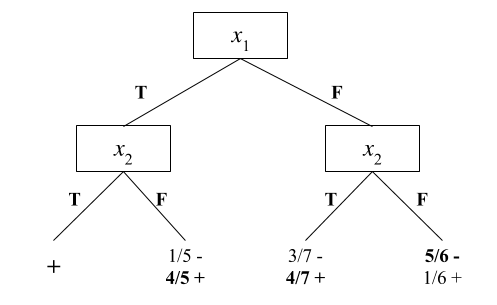
\includegraphics[width=10cm]{InitialTree}
\centering
\end{figure}

In the initial decision tree (Figure 1) the left node under $x_2$ was the only node where the sample population had the same outcome. For all other leaf nodes, we need to select the highest probability of classes in the leaf node population. Doing this for all leaf nodes and collapsing one sub-tree produces the tree in figure 2. The highest probable class (when $x_1 = T$ and $x_2 = F$) is '+' and when $x_1 = T$ and $x_2 = T$ the predicted class is T, so we can collapse the sub-tree under $x_1 = T$ so that whenever $x_1 = T$ our class is '+'.

\begin{figure}[h]
\caption{Final Decision Tree, collapsed left node, select most probable outcome for other nodes.}
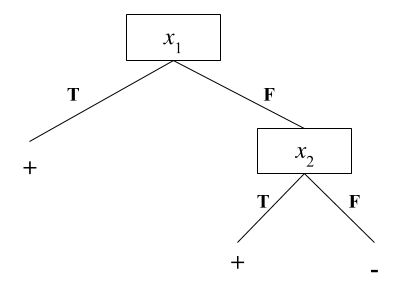
\includegraphics[width=10cm]{FinalTree}
\centering
\end{figure}
\newpage
\end{enumerate}
	
\item We decided that maybe we can use the number of characters and the average word length an essay to determine if the student should get an $A$ in a class or not.  Below are five samples of this data:
\begin{table}[h]
\begin{center}
\begin{tabular}{|l|l|l|}
\hline
\# of Chars & Average Word Length & Give an A\\
\hline
216 & 5.68 & Yes\\
69 & 4.78 & Yes\\
302 & 2.31 & No \\
60 & 3.16 & Yes \\
393 & 4.2 & No\\
\hline
\end{tabular}
\end{center}
\end{table}
\begin{enumerate}
\item What are the class priors, $P(A=Yes), P(A=No)$? (1pt)
\\
\begin{equation*}
\begin{split}
Total Number Samples = 5\\
Number Yes = 3\\
Number No = 2\\
P(A = Yes) = \frac{3}{5}\\
P(A = No) = \frac{2}{5}
\end{split}
\end{equation*}
\newpage
\item Find the parameters of the Gaussians necessary to do Gaussian Naive Bayes classification on this decision to give an A or not.  Standardize the features first over all the data together so that there is no unfair bias towards the features of different scales (5pts).
\\
\begin{flalign*}
Features &= 
\begin{bmatrix}
 216 & 5.68 \\
 69 & 4.78 \\
 302 & 2.31 \\
 60 & 3.16 \\
 393 & 4.2
\end{bmatrix} &\\
\mu &= \begin{bmatrix} 208 & 4.03 \end{bmatrix} &\\
\sigma &= \begin{bmatrix} 145.22 & 1.33 \end{bmatrix}
\end{flalign*}
\begin{flalign*}
Standardized Features &= (Features - \mu) / \sigma = 
\begin{bmatrix}
 0.06  & 1.24 \\
 -0.96 & 0.56 \\
 0.65  & -1.29 \\
 -1.02 & -0.65\\
 1.27  & 0.13
\end{bmatrix}
\end{flalign*}
\begin{flalign*}
\hat{\mu}_{1Y} &= \frac{1}{3}\cdot(0.06-0.96-1.02) &\\
		        &= \frac{-1.92}{3} &\\
		        &= \textbf{-0.64}
\end{flalign*}
\begin{flalign*}
\hat{\sigma}_{1Y} &= \frac{1}{3 - 1}\cdot((0.06+0.64)^2+(-0.96+0.64)^2+(-1.02+0.64)^2) &\\
					 &= \frac{1}{2}\cdot(0.49 + 0.1 + 0.14) &\\
		            &= \frac{0.73}{2} &\\
		            &= \textbf{0.37}
\end{flalign*}
\begin{flalign*}
\hat{\mu}_{1N} &= \frac{1}{2}\cdot(0.65+1.27) = \frac{1.92}{2} = \textbf{0.96} &\\
\end{flalign*}
\begin{flalign*}
\hat{\sigma}_{1N} &= \frac{1}{2 - 1}\cdot((0.65-0.96)^2+(1.27-0.96)^2) &\\
					 &= \frac{1}{1}\cdot(0.1 + 0.1) = \textbf{0.2}
\end{flalign*}

\begin{flalign*}
\hat{\mu}_{2Y} &= \frac{1}{3}\cdot(1.24+0.56-0.65) &\\
		        &= \frac{1.15}{3} &\\
		        &= \textbf{0.38}
\end{flalign*}
\begin{flalign*}
\hat{\sigma}_{2Y} &= \frac{1}{3 - 1}\cdot((1.24-0.38)^2+(0.56-0.38)^2+(-0.65-0.38)^2) &\\
					 &= \frac{1}{2}\cdot(0.74 + 0.03 + 1.03) &\\
		            &= \frac{1.83}{2} &\\
		            &= \textbf{0.92}
\end{flalign*}
\begin{flalign*}
\hat{\mu}_{2N} &= \frac{1}{2}\cdot(-1.29+0.13) = \frac{-1.13}{2} = \textbf{-0.57} &\\
\end{flalign*}
\begin{flalign*}
\hat{\sigma}_{2N} &= \frac{1}{2 - 1}\cdot((-1.29+0.57)^2+(0.13+0.57)^2) &\\
					 &= \frac{1}{1}\cdot(0.52 + 0.49) = \textbf{1.01}
\end{flalign*}
The final inputs for the Gaussians are:\\
\textbf{$F_1$ = Number of characters}\\
\begin{tabular}{ll}
For A = Y & For A = N \\
$\hat{\mu}_{1Y} = -0.64$ & $\hat{\mu}_{1N} = 0.96$ \\
$\hat{\sigma}_{1Y} = 0.37$ & $\hat{\mu}_{1N} = 0.2$ \\
\end{tabular}
\\
\\
\textbf{$F_2$ = Average Word Length}\\
\begin{tabular}{ll}
For A = Y & For A = N \\
$\hat{\mu}_{2Y} = 0.38$ & $\hat{\mu}_{2N} = 0.57$ \\
$\hat{\sigma}_{2Y} = 0.92$ & $\hat{\mu}_{2N} = 1.01$ \\
\end{tabular}
\newpage
\item Using your response from the prior question, determine if an essay with 242 characters and an average word length of 4.56 should get an A or not (5pts).
\begin{enumerate}
\item Standardize Input
\begin{flalign*}
Standardized &= \left(\begin{bmatrix}242 & 4.56\\ \end{bmatrix} - \begin{bmatrix}208 & 4.03\\ \end{bmatrix}\right) / \begin{bmatrix}
145.22 & 1.33\\ \end{bmatrix} &\\
 &= \begin{bmatrix} \frac{34}{145.22} & \frac{0.53}{1.33} \\ \end{bmatrix} &\\
 &= \begin{bmatrix} 0.23 & 0.4 \\ \end{bmatrix}
\end{flalign*}
\item Find $P(A = Y | F_1 = 0.23, F_2 = 0.4)$
\begin{flalign*}
 &= P(A = Y | F_1 = 0.23 | A = Y)\cdot P(F_2 = 0.4 | A = Y) & \\
 &= \frac{3}{5}\cdot\frac{1}{\hat{\sigma}_{1Y}\sqrt{2\pi}}e ^{-\frac{\left(F_1-\hat{\mu}_{1Y}\right)^2}{2 \hat{\sigma}_{1Y}^{2}}}\frac{1}{\hat{\sigma}_{2Y}\sqrt{2\pi}}e ^{-\frac{\left(F_2-\hat{\mu}_{2Y}\right)^2}{2 \hat{\sigma}_{2Y}^{2}}}
 &\\
 &= \frac{3}{5}\cdot\frac{1}{-0.37\sqrt{2\pi}}e ^{-\frac{\left(0.23+0.64\right)^2}{2 \cdot 0.37^{2}}}\cdot\frac{1}{0.92\sqrt{2\pi}}e ^{-\frac{\left(0.4-0.38\right)^2}{2 \cdot 0.92^{2}}}
 &\\
 &= \frac{3}{5}\cdot\frac{1}{-0.37\cdot 2.51}e ^{-\frac{0.76}{0.27}}\cdot\frac{1}{0.92\cdot 2.51}e ^{-\frac{0.02}{1.69}}
 &\\
 &= \frac{3}{5}\cdot\left(\frac{1}{1.93}\cdot 0.05\right)\cdot\left(\frac{1}{2.31}\cdot 1\right)
 &\\
 &= 0.6\cdot \left(1.08 \cdot 0.05\right) \cdot 0.43 = \textbf{0.1}
 &\\
\end{flalign*}
Given that there is 10\% chance of getting an A given this input, it is unlikely this input will produce an A.
\end{enumerate}
\end{enumerate}
\item Consider the following questions pertaining to a k-Nearest Neighbors algorithm (1pt each = 3pts):
\begin{enumerate}
\item How could you use a \emph{validation set} to determine the user-defined parameter $k$?
\\
\\
You can vary $k$ using the training set; then test against the validation set.We will produce a ROC curve with the results when evaluating the validation set.When we achieve a sharp change between $k-values$, we can pick the $k-value$ that worked best on the validation set, before the sharp change in precision/recall.
\item Why shouldn't you use the training set to determine this?
\\
\\
The training set cannot be used to determine the $k-value$ because for k-NN, the training set is the model. The only way to even possibly use the training set is to add one point from the training set (at at time) to the scene and determine the ideal $k-value$. However, this changes the model for every point added.
\item Why shouldn't you use the testing set to determine this?
\\
\\
The reason is similar to never using the test data in training/tuning of a model. There is a high likelihood that the model would be tuned and in a sense 'overfit' or 'over-tuned' to the test data. It would then not be able to generalize to real data, never seen during the training phase.
\end{enumerate}
\item The Linear Kernel is commonly used if we already are working in high feature space.  It is defined as $k(x,y)=\sum_{d=1}^D x_d y_d$.  If your observations have three features ($D=3$), what is the function $\phi(u)$ such that $k(x,y)=\phi(x)\phi(y)$?  Show your work (4pts).
\begin{flalign*}
\kappa(x, y) &= \sum_{d}^{D=3}x_dy_d &\\
					&= x_1y_1 + x_2y_2 + x_3y_3 &\\
\end{flalign*}
\begin{equation*}
\phi(u) = <u_1, u_2, u_3>
\end{equation*}
While, the question asks us to find a function $\phi(u)$ such that we can compute $\kappa(x, y) = \phi(x)\phi(y)$, when the linear kernel is actually used, we instead compute $\kappa(x, y) = \phi(x)^T\phi(y)$. This fact of using the transpose of one of the functions produces the summation above.
\item True or false:  A Gaussian Kernel is better than a linear kernel when there are many features but few training samples (1pt).
\\
\\
\textbf{False}; Assuming more features than samples, we won't benefit from higher-dimensional space. Using a gaussian kernel would project the few samples we do have into an even higher dimensional space. If we have fewer samples than we do dimensions, it is likely we do not have enough data to represent all of the possible 'places' in that higher dimensional space, and therefore we cannot build an accurate model. Instead, we should try to combine or reduce our dimensions so that we have a richer, fuller data set.
\end{enumerate}

\newpage
\section{Naive Bayes Classifier}\label{naive}
Using an implementation of the Naive Bayes classifier, I was able to produce the following statistics.\\
This run used $\frac{2}{3}$ of the data as training data (3067 samples) and $\frac{1}{3}$ for testing (1534 samples). \\

\begin{tabular}{lll}
\textbf{Metrix} & \textbf{Percent} & \textbf{Raw Value} \\
Precision & 62\% & 0.623620309051\\
Recall & 48\% & 0.478003384095 \\
F-measure & 54\% & 0.541187739464\\
Accuracy & 77\% & 0.770534550196
\end{tabular}

\section{Multi-Class Support Vector Machines}\label{svm}
For the support vector machine, the SVC implementation from scikit-learn (\url{http://scikit-learn.org/stable/modules/generated/sklearn.svm.SVC.html#sklearn.svm.SVC}) was used as the implementation. \\
The input used $\frac{2}{3}$ of the data as training (1417 samples) and $\frac{1}{3}$ as test (709 samples). Since we were evaluating multi-class output, both 1-vs-1 and 1-vs-others methods were used.\\
\hfill\linebreak
\textbf{Results from one-vs-others}
Accuracy (1 vs [2, 3]): 84\% (0.840620592384)\\
Accuracy (2 vs [1, 3]): 51\% (0.514809590973)\\
Accuracy (3 vs [1, 1]): 49\% (0.490832157969)\\
\hfill\linebreak
\textbf{Results from one-vs-one}
Accuracy: 92\% (0.919605077574)
\end{document}
